\documentclass[10pt]{article}
\usepackage[landscape]{geometry}
\usepackage{tikz}
\usepackage{graphicx}
\usepackage{comment}
\usetikzlibrary{shapes.misc, positioning}
\usepackage[utf8]{inputenc}
\usepackage{amsmath, amssymb, latexsym}
\usepackage{sidecap}
\usetikzlibrary{decorations.pathreplacing}

\begin{document}
	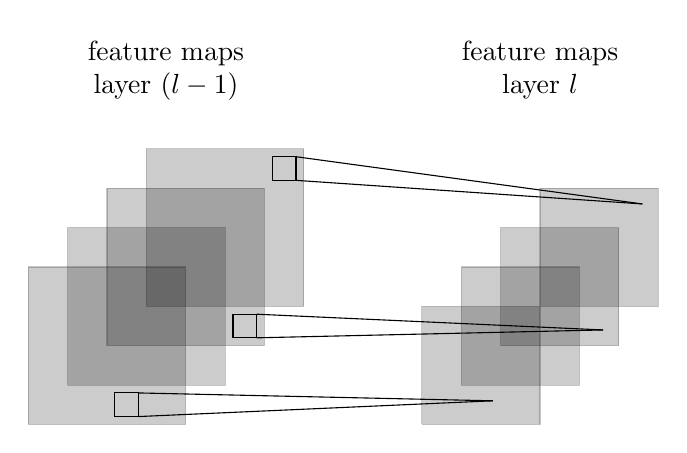
\begin{tikzpicture}
		\node at (1.75,4.5){\begin{tabular}{c}feature maps\\layer $(l-1)$\end{tabular}};
		
		\draw[fill=black,opacity=0.2,draw=black] (1.5,1.5) -- (3.5,1.5) -- (3.5,3.5) -- (1.5,3.5) -- (1.5,1.5);
		\draw[fill=black,opacity=0.2,draw=black] (1,1) -- (3,1) -- (3,3) -- (1,3) -- (1,1);
		\draw[fill=black,opacity=0.2,draw=black] (0.5,0.5) -- (2.5,0.5) -- (2.5,2.5) -- (0.5,2.5) -- (0.5,0.5);
		\draw[fill=black,opacity=0.2,draw=black] (0,0) -- (2,0) -- (2,2) -- (0,2) -- (0,0);
		
		\draw (3.1,3.1) -- (3.4,3.1) -- (3.4,3.4) -- (3.1,3.4) -- (3.1,3.1);
		\draw (2.6,1.1) -- (2.9,1.1) -- (2.9,1.4) -- (2.6,1.4) -- (2.6,1.1);
		\draw (1.1,0.1) -- (1.4,0.1) -- (1.4,0.4) -- (1.1,0.4) -- (1.1,0.1);
		
		\draw (3.4,3.4) -- (7.8,2.8);
		\draw (3.4,3.1) -- (7.8,2.8);
		
		\draw (2.9,1.4) -- (7.3,1.2);
		\draw (2.9,1.1) -- (7.3,1.2);
		
		\draw (1.4,0.4) -- (5.9,0.3);
		\draw (1.4,0.1) -- (5.9,0.3);
		
		\node at (6.5,4.5){\begin{tabular}{c}feature maps\\layer $l$\end{tabular}};
		
		\draw[fill=black,opacity=0.2,draw=black] (6.5,1.5) -- (8,1.5) -- (8,3) -- (6.5,3) -- (6.5,1.5);
		\draw[fill=black,opacity=0.2,draw=black] (6,1) -- (7.5,1) -- (7.5,2.5) -- (6,2.5) -- (6,1);
		\draw[fill=black,opacity=0.2,draw=black] (5.5,0.5) -- (7,0.5) -- (7,2) -- (5.5,2) -- (5.5,0.5);
		\draw[fill=black,opacity=0.2,draw=black] (5,0) -- (6.5,0) -- (6.5,1.5) -- (5,1.5) -- (5,0);
	\end{tikzpicture}
    
     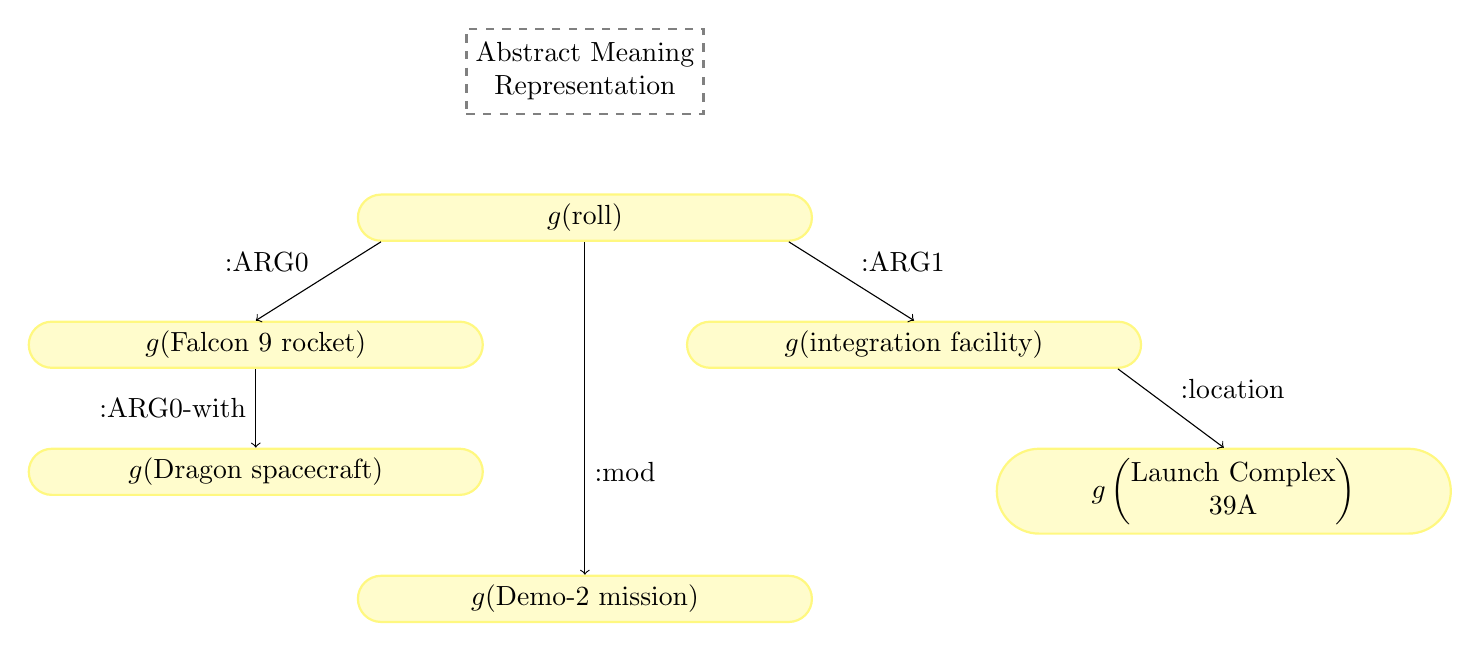
\begin{tikzpicture}
    \tikzset{layer/.style={rectangle,draw=blue!50,fill=blue!20,thick,minimum width=2cm}},
    \tikzset{feature/.style={rectangle,draw=black!50,fill=white, thick}}
    \tikzset{label/.style={draw=white,fill=white}}
    \tikzset{embed/.style={rounded rectangle, draw=yellow!50,fill=yellow!20,thick,minimum width=6cm}}
    % Input image
    % \begin{scope}[node distance=3cm]
    % \node[feature, dashed] (in tag) at (0, 5) {Input image};
    % \end{scope}
    
    % \begin{scope}[node distance=1cm]
    % \node[below=of in tag] (in) {\includegraphics[scale=0.2]{fig1}};
    % \node[layer, rotate=90, below left=of object embed] (object detector) {Object detector};
    % \end{scope}
    
    % Embedding
    \begin{scope}[node distance=1cm and -1cm]
    \node[feature, dashed] (amr) at (3, 0) {\begin{tabular}{@{}c@{}}
         Abstract Meaning\\
         Representation
    \end{tabular}};
    \node[embed, below=of amr] (g1) {$g(\text{roll})$};
    \node[embed, below left=of g1] (g2) {$g(\text{Falcon 9 rocket})$};
    \node[embed, below right=of g1] (g3) {$g(\text{integration facility})$};
    \node[embed, below=of g2] (g4) {$g(\text{Dragon spacecraft})$};
    \node[embed, below right=of g3] (g5)
    {$g\left(\text{\begin{tabular}{@{}c@{}}
         Launch Complex\\
         39A
    \end{tabular}}\right)$};
    \node[embed, below right=of g4] (g6) {$g(\text{Demo-2 mission})$};
    \end{scope}
    
    \draw[->] (g1.south west) -- (g2.north) node[midway, above left] {:ARG0};
    \draw[->] (g1.south east) -- (g3.north) node[midway, above right] {:ARG1};
    \draw[->] (g1.south) -- (g6.north) node[near end, above right] {:mod};
    \draw[->] (g2.south) -- (g4.north) node[near start, below left]{:ARG0-with};
    \draw[->] (g3.south east) -- (g5.north) node[midway, above right]{:location};
    % Label matrix
    % \draw (h4.east) grid ++(4, 4); 
    % \filldraw[black] (7, 3) rectangle ++(1, 1);
    % \filldraw[black] (8, 2) rectangle ++(1, 1);
    % \filldraw[black] (9, 3) rectangle ++(1, 1);
    % \filldraw[black] (9, 1) rectangle ++(1, 1);
    % \filldraw[black] (10, 0) rectangle ++(1, 1); 
    
    % Dot product
    % \draw (13, 1) circle [radius=0.7];
    % \draw (12.5, 0.5) -- ++(1, 1);
    % \draw (12.5, 1.5) -- ++(1, -1);
    \end{tikzpicture}
    
    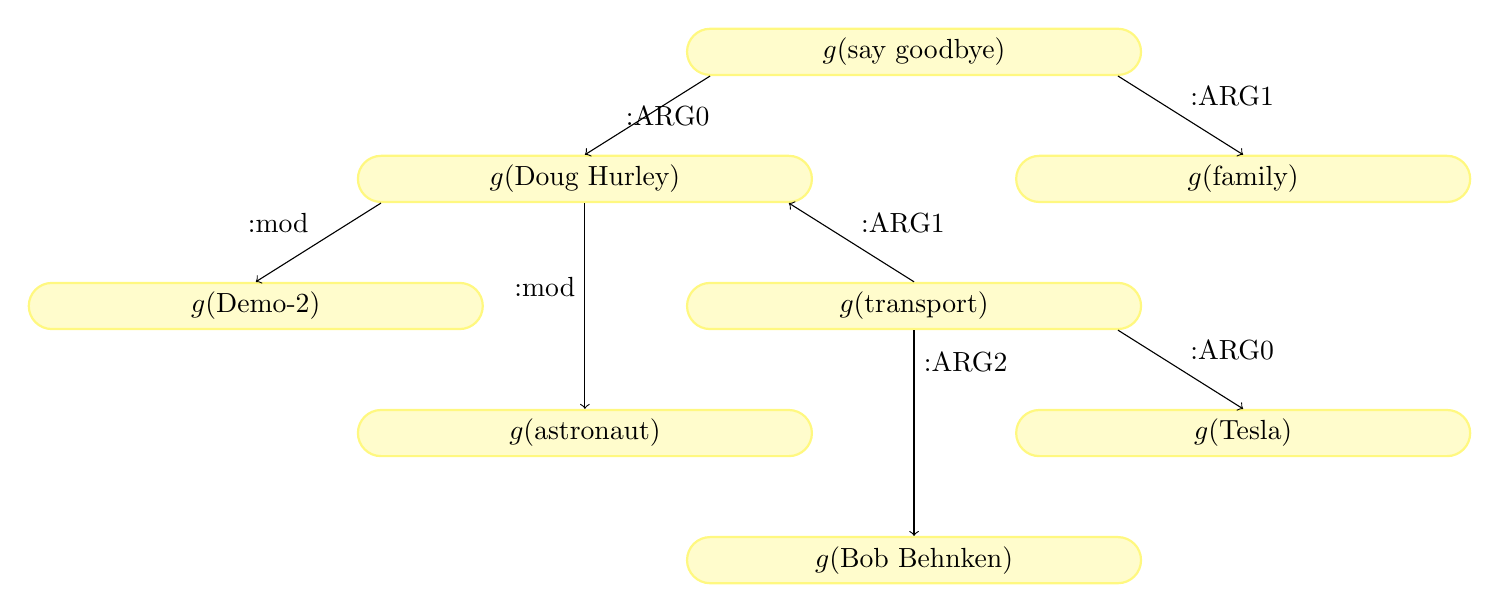
\begin{tikzpicture}
    \tikzset{layer/.style={rectangle,draw=blue!50,fill=blue!20,thick,minimum width=2cm}},
    \tikzset{feature/.style={rectangle,draw=black!50,fill=white, thick}}
    \tikzset{label/.style={draw=white,fill=white}}
    \tikzset{embed/.style={rounded rectangle, draw=yellow!50,fill=yellow!20,thick,minimum width=6cm}}
    \begin{scope}[node distance=1cm and -1cm]
    \node[embed] at (5, 5) (g7) {$g(\text{say goodbye})$};
    \node[embed, below left=of g7] (g8) {$g(\text{Doug Hurley})$};
     \node[embed, below left=of g8] (g13) {$g(\text{Demo-2})$};
    \node[embed, below right=of g7] (g9) {$g(\text{family})$};
    \node[embed, below left=of g9] (g10) {$g(\text{transport})$};
    \node[embed, below left=of g10] (g14) {$g(\text{astronaut})$};
    \node[embed, below right=of g10] (g11) {$g(\text{Tesla})$};
    \node[embed, below left=of g11] (g12) {$g(\text{Bob Behnken})$};
    \end{scope}
    
    \draw[->] (g7.south west) -- (g8.north) node[near end, above right] {:ARG0};
    \draw[->] (g7.south east) -- (g9.north) node[midway, above right] {:ARG1};
    \draw[->] (g8.south west) -- (g13.north) node[midway, above left] {:mod};
    \draw[->] (g8.south) -- (g14.north) node[midway, above left] {:mod};
    \draw[->] (g10.north) -- (g8.south east) node[midway, above right] {:ARG1};
    \draw[->] (g10.south east) -- (g11.north) node[midway, above right] {:ARG0};
    \draw[->] (g10.south) -- (g12.north) node[near start, above right] {:ARG2};
     
    \end{tikzpicture}
    
\tikzstyle{every picture}+=[remember picture]
\tikzstyle{na} = [shape=rectangle,inner sep=0pt,text depth=0pt]
\tikz\node[na](word1){John}; loves \tikz\node[na](word2){his}; mother.
\begin{tikzpicture}[overlay]
  \path[->,red,thick](word2) edge [out=90, in=90] (word1);
\end{tikzpicture}
\\\\


\tikzstyle{every picture}+=[remember picture]
\tikzstyle{ann} = [shape=rectangle, inner sep=0pt, text depth=0pt]
\tikzset{square arrow/.style={to path={-- ++(0,.5) -| (\tikztotarget)}}}

\tikz\node [ann, fill=white, draw=blue!40, thick](e1) {IBM Research – Brazil}; is one of twelve research laboratories comprising \tikz\node [ann, fill=white, draw=blue!80, thick] (e2) {IBM Research};,

its first in \tikz\node (e3) [ann, fill=white, draw=purple!60, thick] {South America};. It was established in \tikz\node (e4) [ann, fill=white, draw=green!90, thick] {June 2010}; , with locations in \tikz\node (e5) [ann, draw=yellow!90, thick] {S\u00e3o Paulo};

and \tikz\node (e6) [ann, draw=orange!60] {Rio de Janeiro};.
\end{document}